\section{Foundations}
\label{sec:foundation}

Originally, OCL was designed as a constraint language for UML. Recent work showed
that OCL can be applied to various other modelling and meta-modelling languages. Thus,
an abstract description of OCL and its relation to modelling languages is sensible.

\subsection{The Generic Three Layer Architecture}
As discussed in \cite{demuthRGWS09}, OCL evaluation
always involves three adjacent layers of the \emph{MOF four layer metadata
architecture} \cite{spec:MOF1-4}. This leads to the notion of 
a \emph{generic three layer architecture} for OCL as depicted in
Fig.~\ref{fig:genericlayers}~(a). 
At layer Mn+1, OCL is bound to a concrete modelling language that has to provide 
concepts like
types, navigable properties, and possibly operations. 
This binding allows the definition of
OCL constraints on models that are described by the meta-model (Mn layer).
During the evaluation of these constraints, an OCL interpreter has to query model
instance elements for their properties or invoke operations on them ({Mn-1} layer).

Model instances are often realised in
a different \emph{technological space}~\cite{kurtev2002technological} than their model. Then, there are two model
representations at the layer Mn (cf. Fig.~\ref{fig:genericlayers}~(a)): the original constrained \emph{model} and a
\emph{model realisation} implementing the model in a specific technological space. The
model realisation is typically derived by a transformation of the model
\cite{WWW:EMF}. 
This leads to the problem that the connection between the different model representations
at the Mn layer is hidden inside the transformation and may not be accessible from the OCL infrastructure.
An algorithm matching the elements of the model realisation and the constrained model can re-establish
this connection.
% \remove{ can be obtained by a
% \emph{Reflection} \cite{smith1982procedural} mechanism of the model instance.}
%Since constraints are defined on the original model but evaluated on
%instances of the model realisation, there has to be a matching of elements in
%the original model and of the model realisation. 

% sorry had to restructure the prev. paragraph and exact change tracking was to
% complicated

	\begin{figure}[t]
			\centering
				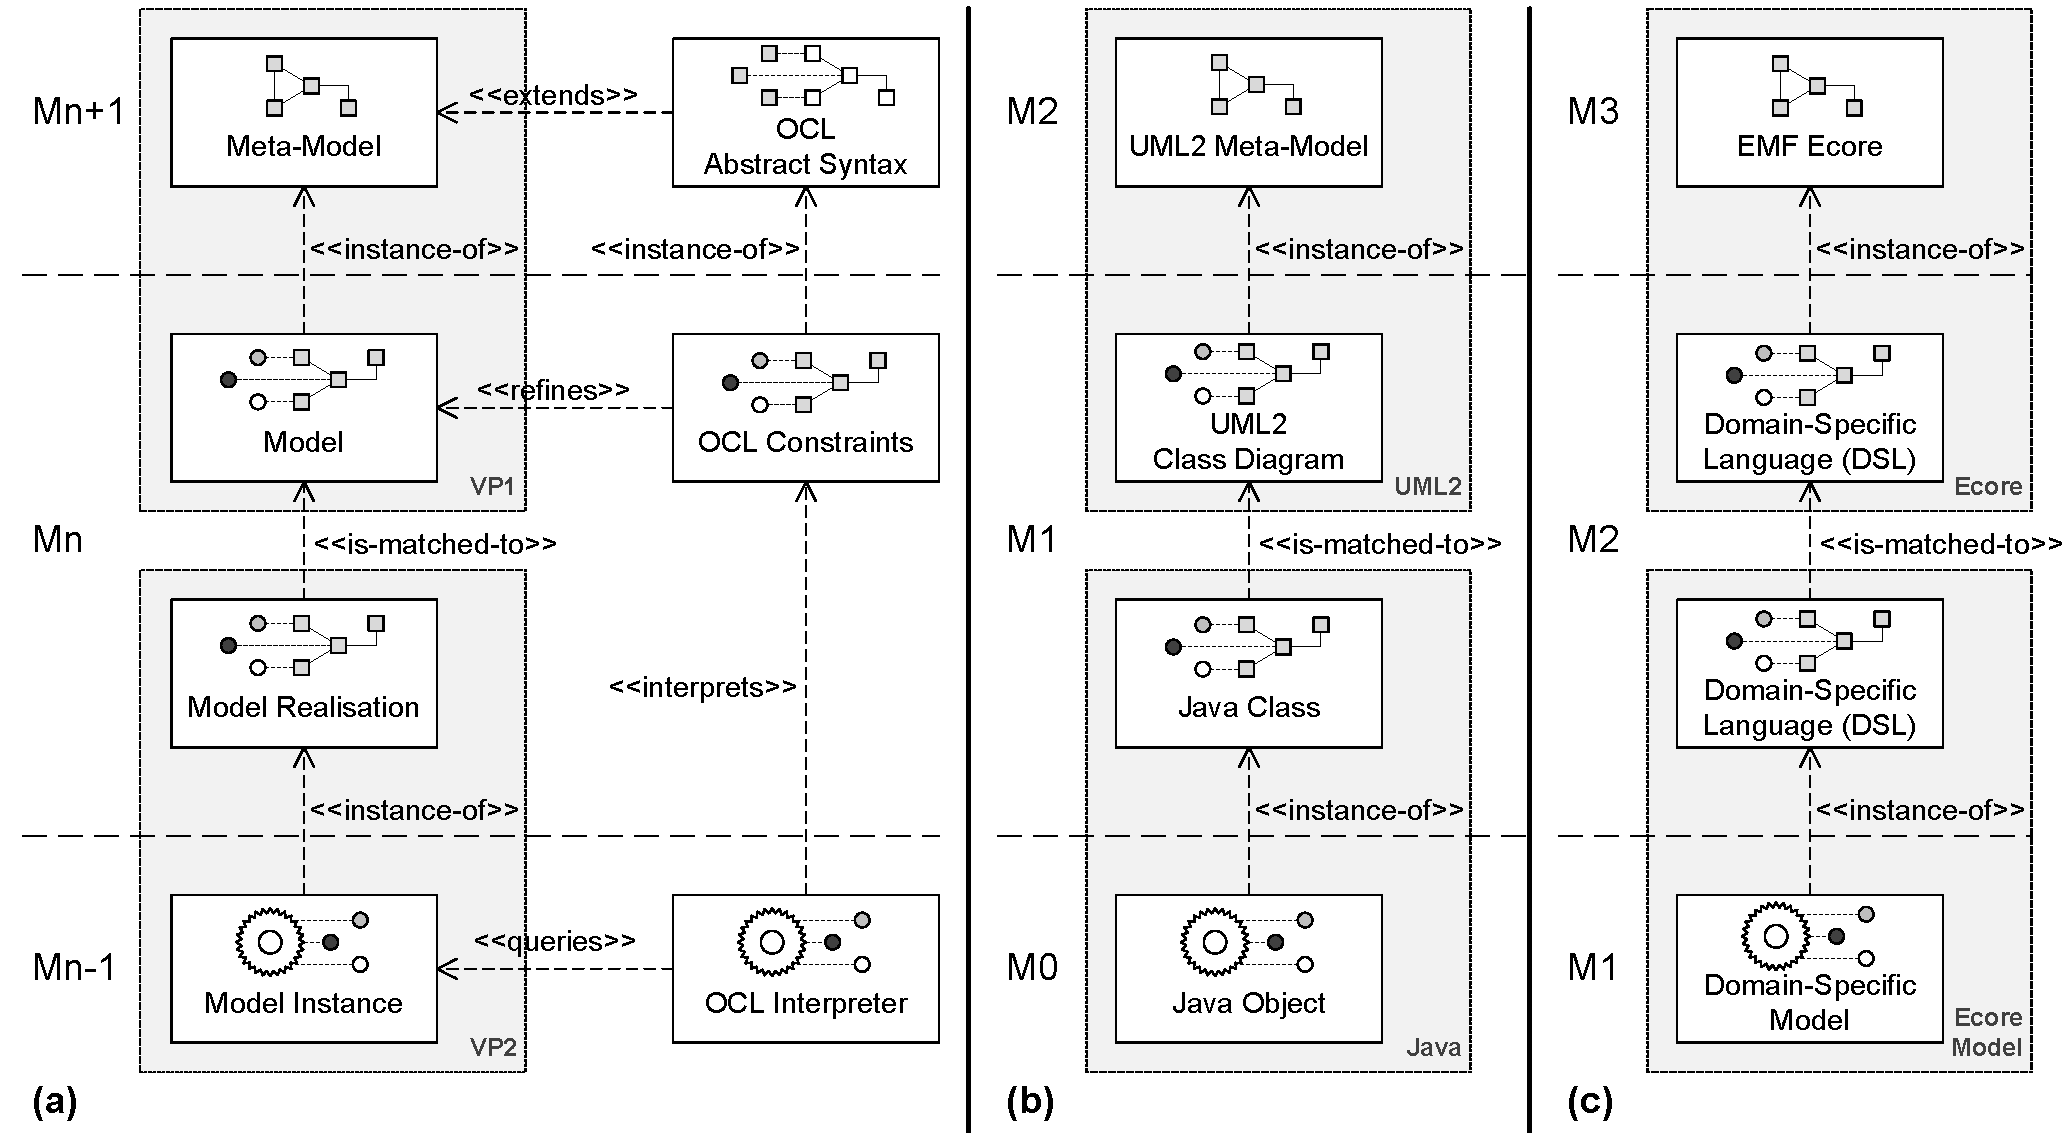
\includegraphics[width=1.00\textwidth]{figures/genericlayers.pdf}
			\caption{The Generic Three Layer Architecture}
			\label{fig:genericlayers}
		\end{figure}
	%\note{Fig 1. add headings to subfigures: a) Variation points in OCL Application	b) Applciation of OCL in UML modeling c) Application of OCL in Ecore
	%metamodeling } 


Instances of this generic three layer architecture are shown in
Fig.~\ref{fig:genericlayers}~(b) and (c). Fig.~\ref{fig:genericlayers}~(b)
exemplifies the application of OCL to constrain UML class diagrams. At M2 (Mn+1) 
the OCL abstract syntax is bound to the UML meta-model. At M1 (Mn) constraints are defined against UML
class diagrams. At this layer the original UML model is transformed to a
Java-based model representation where UML classes correspond to Java classes.
At M0 (Mn-1) the OCL constraints are evaluated against Java
objects.

The example in Fig.~\ref{fig:genericlayers} (c) demonstrates the
application of OCL constraints to define well-formedness rules (WFRs) for
DSLs built with EMF Ecore. The generic three layer architecture is lifted one
layer: At M3 (Mn+1) the OCL abstract syntax is bound to the Ecore
meta-meta-model. At M2 (Mn) a new DSL is defined using Ecore and OCL-based WFRs. 
Since EMF contributes a runtime infrastructure for models
and model instances no transformation is required at M2. The model and the
model representation are identical. At M1 (Mn-1) the WFRs are
evaluated against models built with the defined DSL.
% Here, the model is a domain-specific language
% modelled in Ecore (M2) for which WFRs are evaluated on domain-specific models (M1). In this case, the model and its realisation are identical.

\subsection{Variation Points of OCL Interpretation}

With instantiation of our generic three layer architecture for various OCL
applications found in literature, we identified
two variation points. The first variation point (VP1) describes variability at Mn+1 and Mn
w.r.t. the modelling language used to specify constrained models. The second variation point (VP2)
relates to variability at Mn and Mn-1 t w.r.t. the technological space
model instances are realised and validated in (cf. Fig.~\ref{fig:genericlayers}
(a)). 
% In the feature model two
% variation points regarding OCL interpretation can be identified: constrained models (VP1) as well as model instances (VP2) can vary.

With the generic three layer architecture it is possible to vary several
models and model instances independently. For example the same UML model can be
combined with OCL evaluation on model instances realised in Java or a
relational database, or the OCL evaluation on XML-based model instances can be
used for models built with the UML or the Ecore meta-model. The feature model
depicted in Fig.~\ref{fig:features} documents the variation space of OCL
applications found in literature. The only constraint
a variant configuration of the generic architecture has to
satisfy is that the model instance bound to VP2 is located exactly one
meta-layer below the model bound to VP1. 

  \begin{figure}[t]
			\centering
		  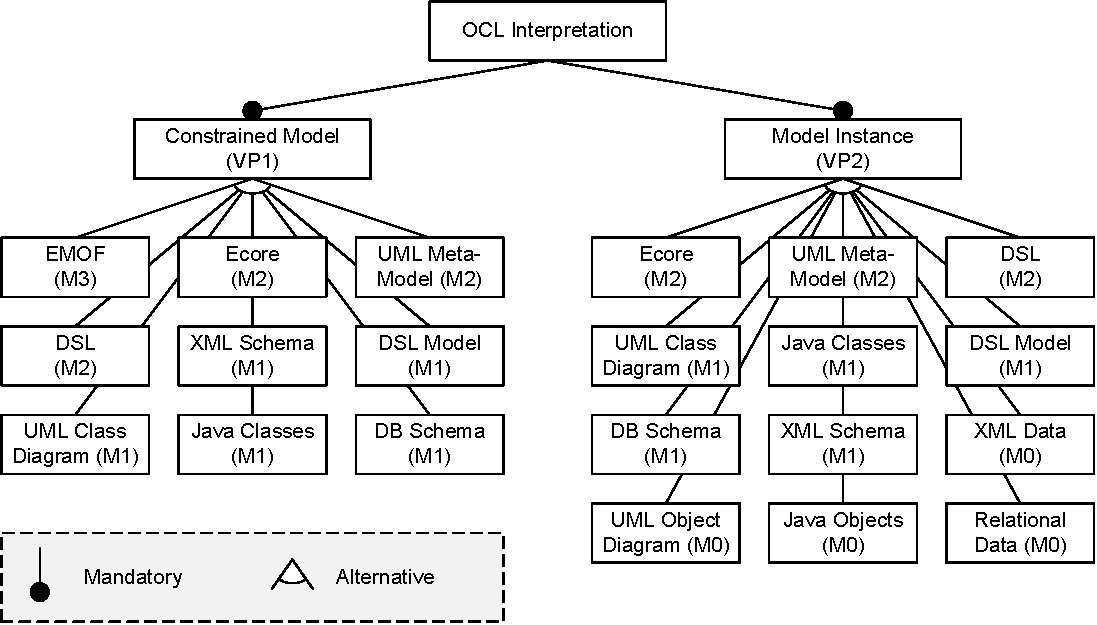
\includegraphics[width=1.00\textwidth]{figures/features.pdf}
			\caption{Features of OCL Interpretation}
			\label{fig:features}
	\end{figure}
	
Several OCL tools provide
support for variation on VP1
\cite{WWW:MDT,akehurst2003ocl,WWW:dresdenOCL,kolovos2008detecting}. 
Yet, those tools do not address VP2 as their supported models require specific 
instances (typically both located in the same technological space).
We argue that this tight coupling can be reduced to avoid the
reimplementation of OCL interpreters for different technological spaces.
In the following we contribute an implementation of the generic three layer
architecture that supports VP1 and VP2.

	
	
	
	

% The \textit{Generic Three Layer Meta data Architecture}. (a): Each OCL constraint requires a meta-model defining a model on which OCL constraints are specified. The 
%			constraints are evaluated on a model instance that instantiates the constrained model. 
%			The generic architecture can be parametrized at two different variation points. Different
%			models and their meta-models can be bound to VP1, different model instances can be bound
%			to VP2.	(b): UML-Example for layers M2, M1 and M0. VP1 is bound to the UML meta-model (MOF), 
%			VP2 is bound to Java. (c): EMF-Example for layers M3, M2 and M1. VP1 is bound to EMF Ecore,
%			VP2 is bound to Ecore-based models.
%
%	To differentiate between meta-models, models and runtime objects, the OMG introduced 
%	the \textit{MOF Four Layer Metadata Architecture}, that locates the meta-model, 
%	model, and the model's instances at the layers \textit{M2}, \textit{M1} and \textit{M0}. 
%	\note{Is that important to understand the paper?; Michael: agreed, just refer to it, but leave explaination}{Each language at layer
%	\textit{Mn} is described in terms of a language resided at layer \textit{Mn-1}. Meta-meta-models 
%	that are located at the layer \textit{M3} 
%	can describe themselves reflexively.}
%	
%	Fig.~\ref{fig:genericlayers} depicts the \textit{Generic Three Layer
%	Meta-Data Architecture} aligning OCL constraints with the MOF layers.
%	\remove{As all
%	models can be located in this layer architecture, OCL can be located there as
%	well.} OCL constraints are a model and can be described using their abstract
%	syntax, i.e., the OCL meta-model. They are evaluated for runtime objects at the 
%	model instance layer. 
%	%\remove{Thus, three layers must be known by the OCL tool
%	%to define and evaluate the constraints. This notion leads to the 
%	%Generic Three Layer Meta-Data Architecture demuthRGWS09} that 
%	%allows to define an OCL tool independently of specific layers. As can be seen
%	%in Figure \ref{fig:genericlayers} the OCL model (all constraints) enriches
%	%another model.} 
%	In order to \change{navigate through the  model or to call
%	operations on}{define constraints on models OCL needs to navigate on} model
%	elements. To bind OCL constraints on the navigation structure in
%	the model they are defined on, the abstract syntax of OCL
%	\note{this is true for UML, but sounds quite technical}{extends} the model's
%	meta-model.
%	%OCL can be used to define well-formedness rules, i.e., constraints on meta-models (M2) that are evaluated at the model level (M1), or business rules, i.e., constraints defined on models (M1) that are evaluated for runtime objects at the model instance layer (M0).
%	
%	\note{we need to incorporate the motivation for implementation language
%	variation here. Reviewers need to understand the problem to understand our
%	solution.}
%
%
%	\note{This section does not clarify the contribution of THIS paper. We should
%	sell the instance adaptation as a improvement of previous DresdenOCL versions
%
%	
%	}
%
%	{The architecture of Dresden OCL2 for Eclipse was developed in respect to the 
%	generic three layer meta-data architecture. In order to reuse the developed 
%	OCL tools, DresdenOCL does not directly accesses models or model instance objects. 
%	Instead, these are hidden behind a common set of interfaces that delegate to 
%	their adaptee. The adaptation of models and model instance objects is presented 
%	in the following.}


